\documentclass[dutch]{beamer}
\mode<presentation>

%\documentclass[handout]{beamer}
%\usepackage{pgfpages}
%\pgfpagesuselayout{4 on 1}[a4paper,border shrink=5mm,landscape]
%\setbeamertemplate{footline}[frame number]

\usepackage[dutch]{babel}
\usepackage{graphicx}
\usepackage{amssymb}
\usepackage{subfig}
\usepackage{amsthm}
\usepackage[utf8]{inputenc}
\usepackage[normalem]{ulem}
\usepackage{color}
\usepackage{cancel}
\usepackage{wrapfig}

\newcommand{\vraag}[1]{\begin{itemize}\item[Vraag:] {\it #1}\end{itemize}}
\newcommand{\degree}{\ensuremath{^\circ}}

\graphicspath{{../figuren/}}

\begin{document}
\small

\begin{frame}
 \frametitle{Iets statistisch onderzoeken}
 {\it Onderzoeken} is iets nauwkeurig nazien of nagaan.\\
 {\bf Onderzoeksvraag}: vraag die bij een onderzoek hoort.\\
 {\it Statistisch onderzoek} is een onderzoek die verloopt volgens de statistiek.\\
 {\bf Statistiek} is de wetenschap van het waarnemen van verschijnselen en het weergeven van de uitkomsten in getallen en figuren.\\
 Onderzoek:\\
 \begin{enumerate}
  \item Wat wil je weten? Hoe ga je meten?
  \item Op speurtocht gaan in de dataset.
  \item Wat heb je gevonden? Hoe ver kan je gaan in je conclusie?
  \item Kernachtig samenvatten van onderzoek.
\end{enumerate}
\end{frame}

\begin{frame}
\frametitle{Statistisch onderzoek naar de kleuren van M\&M-snoepjes}
{\bf Onderzoeksvraag:}\\
Heb je enig idee welke kleuren allemaal voorkomen bij M\&M’s?
Komt elke kleur evenveel voor?\\\vspace*{0.5cm}

{\bf Populatie} als je “de totale verzameling” bedoelt.\\
{\bf Steekproef} is een deeltje van een populatie.\\\vspace*{0.5cm}

{\bf Aselecte steekproef}: goed mengen en dan lukraak snoepjes eruit nemen.\\
{\bf Aselect} zijn: elk element van de populatie moet dezelfde kans hebben om opgenomen te worden tot de steekproef.\\
{\bf Representatief} zijn: de steekproef een correct beeld moet geven van de verscheidenheid binnen de populatie.\\
{\bf steekproefgrootte}: aantal gekozen snoepjes.

\end{frame}

\begin{frame}
\frametitle{Gegevensverzameling of dataset}
De {\bf elementen} zijn de objecten die in een statistische studie worden onderzocht (de snoepjes).\\
Elke {\bf veranderlijke} is één welbepaalde eigenschap die je opmeet (de kleur).\\
{\bf Kwalitatieve veranderlijke}: veranderlijke waarop geen zinvolle wiskundige bewerkingen uitgevoerd kunnen worden.\\ 
De {\bf dataset} is een tabel met op de rijen de elementen en in de kolommen de veranderlijken.\\
\vraag{Maak een tabel waarin je de gegevens zal opschrijven. Als je afkortingen gebruikt, schrijf dan ook op wat die afkortingen betekenen.}
\vspace{5cm}
\end{frame}

\begin{frame}
\frametitle{Frequentietabel}
\vraag{Gebruik je dataset om een frequentietabel op te stellen.}
\begin{center}
  \begin{tabular}{|p{2cm}|p{2cm}|p{2cm}|}
    \hline
    \uncover<2->{Kleur}&\uncover<2->{Frequentie}&\uncover<5->{Relatieve Frequentie}\\
    \hline
    &&\vspace*{0pt}\\
    \hline
    &&\vspace*{0pt}\\
    \hline
    &&\vspace*{0pt}\\
    \hline
    &&\vspace*{0pt}\\
    \hline
    &&\vspace*{0pt}\\
    \hline
    &&\vspace*{0pt}\\
    \hline
  \end{tabular}
\end{center}
%\vspace{1cm}
\uncover<3->{\vraag{Hoe kan je de steekproefgrootte snel berekenen met behulp van de frequentietabel?}}
\uncover<4->{\underline{Tel alle frequenties samen} want dan heb je het totale aantal snoepjes en dat is gelijk aan de
steekproefgrootte.}
\end{frame}

\begin{frame}
\frametitle{Relatieve frequentie}
\vraag{Als er in de volledige populatie, dus alle snoepjes in het vat, 6 kleuren zitten. En
van elk kleur zijn er evenveel snoepjes. Wat is dan de kans om lukraak een geel snoepje te kiezen?}
\pause
Van elk kleur zijn er evenveel snoepjes. Dus \uline{elk kleur heeft evenveel kans om gekozen te worden}. Er zijn zes kleuren, dus de kans is $\frac{1}{6}$.
\pause
\vraag{De relatieve frequentie voor "geel" wijkt af van de theoretische kans, verklaar dit en wanneer
zou de relatieve frequentie dichter bij de theoretische kans moeten komen?}
\pause
De relatieve frequentie werd berekend uit een steekproef. \uline{Een steekproef is een lukraak deel van de volledige populatie}. \uline{Hoe groter de steekproef}, hoe dichter we bij de volledige populatie komen en hoe dichter we bij de theoretische kans komen.
\end{frame}

\begin{frame}
\frametitle{Staafdiagram}
Het {\bf Staafdiagram} is de basisfiguur voor kwalitatieve veranderlijken.
Werkwijze:
\begin{enumerate}
  \item Op de $x$-as zet je de verschillende kleuren.
\item Op de $y$-as duid je de frequentie van elke kleur aan en je tekent dan bij elke kleur een staafje
waarvan de lengte overeenkomt met de frequentie van die kleur. Zorg ervoor dat alle staafjes
los van elkaar staan.
\item Voorzie de assen van de juiste naam.
\end{enumerate}
\pause
\vraag{Teken nu zo’n staafdiagram voor het onderzoek.}
\end{frame}


\begin{frame}
\frametitle{Taartdiagram}
Het {\bf Taartdiagram} is bij uitstek bruikbaar om de relatieve frequentie weer te geven.\\
Eén stukje uit een taartdiagram heet een {\bf sector}.\\
Afspraken:
\begin{itemize}
  \item Begin bovenaan en draai met de wijzers van de klok mee.
  \item De grootste sector komt eerst, dan komt de tweede
grootste, enzovoort.
\end{itemize}
\pause
\vraag{Bereken eerst voor elke relatieve frequentie hoe groot de sector is die daarbij hoort.}
\begin{center}
  \begin{tabular}{|p{1cm}|p{1cm}|p{1cm}|p{1cm}|p{1cm}|p{1cm}|p{1cm}|}
    \hline
    kleur:\vspace{0.5cm}&&&&&&\\
    \hline
    hoek:\vspace{0.5cm}&&&&&&\\
    \hline
  \end{tabular}
\end{center}
\pause
\vraag{Teken nu cirkelsectoren die overeenstemmen met de relatieve frequenties.}
\end{frame}

\begin{frame}
\frametitle{Variabiliteit van de steekproefresultaten}
Laten we nu eens kijken naar de inhoud van een aantal andere zakjes M\&M's.\\
\pause
\vraag{Verwacht je dat de andere zakjes dezelfde resultaten zullen hebben als het eerste zakje?}
\pause
\uline{Neen}. Er is \uline{fluctuatie} bij het vullen van de zakjes en dus zullen de antwoorden niet identiek
zijn. Waarschijnlijk lijken de antwoorden wel goed op elkaar, maar anderzijds krijg je snel
“schijnbaar” grote verschillen bij zo’n kleine aantallen. Als er toevallig in een zakje 4
bruine snoepjes zitten en in een ander zitten er 8 bruine, dan is dat plots dubbel zoveel.
\pause
\vraag{Kan je je antwoord op vorige vraag wat verduidelijken door te verwijzen naar de manier
waarop die zakjes gevuld worden? Kan je hierbij ook de woorden populatie en steekproef op
een juiste wijze gebruiken?}
\pause
\uline{Elk zakje kan je beschouwen als een nieuwe steekproef} uit dezelfde grote populatie van alle
M\&M’s. Bij \uline{een steekproef trek je lukraak} en het is dus normaal dat de resultaten van de ene
steekproef niet identiek dezelfde zijn als de resultaten van een andere steekproef.
\end{frame}

\begin{frame}
\frametitle{Variabiliteit van de steekproefresultaten}
In plaats van naar alle kleuren te kijken, zou je er eens je lievelingskleur kunnen uithalen,
bijvoorbeeld blauw.\\
\pause
\vraag{Noteer voor elk onderzocht zakje telkens het percent blauwe snoepjes.}
\vspace*{1cm}
\pause
\vraag{Als jij maar één zakje snoepjes mag onderzoeken (bijvoorbeeld het eerste) en je zou moeten raden hoeveel
percent blauwe snoepjes er door de fabrikant gemaakt wordt (dus hoeveel percent blauwe
snoepjes er in de totale populatie zit), wat zou jij dan antwoorden?}
\vspace*{1cm}
\pause
\vraag{Is je bovenstaand antwoord exact juist? Hoe weet je dat?}
\pause
Neen, want een ander zakje kan een ander aantal blauwe snoepjes bevatten. \uline{Een steekproefuitslag is nooit "wiskundig exact"}! We kunnen enkel een benadering geven.
\end{frame}

\begin{frame}
\frametitle{Steekproefgrootte, nauwkeurigheid en haalbaarheid}
Het is beter om met een grotere steekproef te werken dan met een kleinere. Om een grotere steekproef te krijgen brengen we nu alle open gedane zakjes M\&M's samen en gebruiken we deze als één grote steekproef.
\vraag{De verschillende resultaten van elk onderzocht zakje worden nu verzameld.}
\begin{center}
  \begin{tabular}{|p{2cm}|p{2cm}|p{2cm}|}
    \hline
    Kleur&Frequentie&Relatieve frequentie\\
    \hline
    &&\vspace*{0pt}\\
    \hline
    &&\vspace*{0pt}\\
    \hline
    &&\vspace*{0pt}\\
    \hline
    &&\vspace*{0pt}\\
    \hline
    &&\vspace*{0pt}\\
    \hline
    &&\vspace*{0pt}\\
    \hline
  \end{tabular}
\end{center}
\end{frame}

\begin{frame}
\frametitle{Een model voor de populatie}
Bij M\&M’s komen alle kleuren globaal (in de populatie) evenveel voor.

\vraag{Maak een tabel waarin je aangeeft hoe de populatie er precies uitziet. Gebruik je frequenties
of relatieve frequenties in die tabel?}
\begin{center}
  \begin{tabular}{|p{2cm}|p{2cm}|}
    \hline
    Kleur&\\
    \hline
    &\vspace*{0pt}\\
    \hline
    &\vspace*{0pt}\\
    \hline
    &\vspace*{0pt}\\
    \hline
    &\vspace*{0pt}\\
    \hline
    &\vspace*{0pt}\\
    \hline
    &\vspace*{0pt}\\
    \hline
  \end{tabular}
\end{center}
\end{frame}

\begin{frame}
\frametitle{Een staafdiagram met subgroepen}
\vraag{Hoe ga je de grafiek tekenen? Welke volgorde kies je voor de kleuren op de $x$-as?}
\pause
Om twee situaties met elkaar te vergelijken, ga ik met \uline{relatieve frequenties} werken. Enkel als
ik toevallig even grote subgroepen zou hebben, zou ik ook frequenties kunnen gebruiken.
Voor het staafdiagram met subgroepen plaats ik de \uline{kleuren op de x-as} en de \uline{relatieve
frequenties op de y-as}. Omdat de kleuren van de populatie hier allemaal dezelfde relatieve
frequentie hebben mag ik de volgorde vrij kiezen. Ik zou mij daarbij kunnen laten leiden door
de relatieve frequenties in de steekproef.
\pause
\vraag{Teken nu de grafiek.}
\pause
\vraag{Kan je verklaren waarom jouw cijfers eventueel afwijken van die van de fabrikant?}
\pause
De \uline{cijfers van de fabrikant liggen vast}, want zij beschrijven het model van de totale
populatie. De \uline{cijfers van mijn klas zijn toevallige uitkomsten van een steekproef}. Als wij
volgende week een nieuw onderzoek van M\&M’s zouden doen, dan zouden wij waarschijnlijk
andere resultaten vinden voor onze klas. Maar de cijfers van de fabrikant veranderen niet.
\end{frame}

\begin{frame}
\frametitle{Kernachtige samenvatting van dit onderzoek}
\begin{itemize}
  \item Informatie over het onderzoek.
  \item Antwoorden op de contextvragen.
  \item Besluiten over het uitgevoerde onderzoek.
\end{itemize}
\pause
De contextvragen:
\begin{enumerate}
  \item {\bf Waarom} is dit onderzoek uitgevoerd?
  \item {\bf Waar} is dit onderzoek uitgevoerd?
  \item {\bf Wanneer} is dit onderzoek uitgevoerd?
  \item {\bf Wie of wat} wordt onderzocht?
  \item {\bf Wat} wordt er juist opgemeten?
  \item {\bf Hoe} wordt dit onderzoek uitgevoerd?
\end{enumerate}
\end{frame}

\begin{frame}
\frametitle{Antwoorden op contextvragen}
\vraag{Formuleer in een bondige tekst de antwoorden op de contextvragen.}
\pause
Op \uline{maandag 23 april 2012} hebben we in \uline{onze school} tijdens de les wiskunde een
onderzoek gedaan naar de \uline{kleuren van M\&M-snoepjes}. We wilden weten \uline{welke kleuren}
allemaal voorkwamen en \uline{hoe vaak elke kleur} voorkomt. Voor dit onderzoek hebben we een
aantal zakjes M\&M gebruik. We hebben ook \uline{met de gegevens van de fabrikant rekening gehouden}.
We wilden namelijk de resultaten van onze toevallige steekproef vergelijken met de
populatie-eigenschappen die de fabrikant opgeeft.
\end{frame}

\begin{frame}
\frametitle{Besluiten over het onderzoek}
\vraag{Formuleer in een bondige tekst je besluiten over het uitgevoerde onderzoek.}
\pause
Bij het onderzoeken van de kleuren van M\&M’s hebben we vastgesteld dat er \uline{in elk zakje
dezelfde kleuren voorkomen}, maar \uline{niet allemaal in dezelfde hoeveelheid}. Dit is te verklaren
omdat \uline{zakjes lukraak gevuld} worden. Elk zakje kan beschouwd worden als een lukrake
steekproef uit een enorm grote populatie. Als we alle \uline{zakjes samenvoegen, dan hebben we
een grotere steekproef} maar ook die is te beschouwen als een lukrake steekproef van snoepjes
uit de grote populatie. Het is dus te verwachten dat onze resultaten niet exact samenvallen
met de cijfers die de fabrikant opgeeft.
\end{frame}

\begin{frame}
\frametitle{Zelfevaluatie}
In dit onderzoek heb je geleerd over:\\
\begin{itemize}
  \item de context van een statistisch onderzoek (wanneer, waar,...)
  \item het onderscheid tussen de populatie en een steekproef
  \item een aselecte steekproef
  \item de structuur van een dataset (elementen, veranderlijken)
  \item kwalitatieve veranderlijken
  \item de frequentietabel bij een kwalitatieve veranderlijke
  \item het staafdiagram bij een kwalitatieve veranderlijke
  \item het taartdiagram bij een kwalitatieve veranderlijke
\end{itemize}
\end{frame}

\begin{frame}
\frametitle{Opdrachten}
\vraag{Zeg in eigen woorden op welke vragen je een antwoord moet kunnen geven als men vraagt
naar de context van een statistisch onderzoek.}
\pause
Een verslag moet samen met de bedoeling (\uline{waarom?}) van een statistisch onderzoek ook de
omstandigheden vermelden waarin dit onderzoek is uitgevoerd. Dat betekent dat je plaats
(\uline{waar?}) en tijd (\uline{wanneer?}) moet aangegeven, samen met de manier waarop de steekproef is
getrokken (\uline{hoe?}) en wat er daarna bij wie is opgemeten.
\pause
\vraag{Omschrijf de begrippen steekproef en populatie in je eigen woorden en geef een (nieuw)
voorbeeld. Leg voor jouw voorbeeld uit hoe je daar een aselecte steekproef zou
trekken.}
\pause
Een \uline{populatie is het grote geheel waarover je iets wil weten}. Een \uline{steekproef is een klein
deeltje uit die populatie}. Als ik wil weten of 16-jarige Vlaamse jongeren voor of tegen
huiswerk zijn, dan bestaat de populatie die ik onderzoek uit alle 16-jarige Vlaamse jongeren.
Om hieruit een enkelvoudige aselecte steekproef te trekken, zou ik al die jongeren een
nummer geven en dan 100 toevalsgetallen gebruiken om een steekproef van 100 jongeren te
trekken. In de praktijk is dit geen eenvoudige opdracht.
\end{frame}

\begin{frame}
\frametitle{Opdrachten {\smallskip (vervolg)}}
\vraag{Leg duidelijk uit hoe een dataset eruitziet. Gebruik hiervoor een nieuw voorbeeld dat je zelf
hebt bedacht.}
\pause
In een dataset verzamel je de onderzoeksgegevens. \uline{Per onderzochte persoon (of voorwerp)
maak je een rij in een tabel. Dit zijn de elementen.} Bij elk element meet je één of meerdere
dingen op. Dit zijn \uline{de veranderlijken. Die worden in de kolommen geschreven.}
Als je wil weten wat het merk is van de lievelingsfrisdrank van de leerlingen van je school,
dan kan je eerst een lukrake steekproef van 30 leerlingen trekken. Dat zijn de elementen van
je dataset en dus de 30 rijen in je tabel. Per leerling kan je dan bijvoorbeeld de naam, de klas
en het merk noteren. Dat zijn dan 3 veranderlijken per element en die komen in de 3
kolommen van je dataset terecht.
\pause
\vraag{Zeg in eigen woorden wanneer je over een kwalitatieve veranderlijke spreekt. Is de bloedgroep zo’n veranderlijke? Kan je zelf een kwalitatieve veranderlijke bedenken?}
\pause
Een \uline{kwalitatieve veranderlijke is een veranderlijke waarmee met de mogelijke uitkomsten
geen zinvolle wiskundige bewerkingen kunnen gedaan worden}. De bloedgroep van een
persoon is een goed voorbeeld van een kwalitatieve veranderlijke.
\end{frame}

\begin{frame}
\frametitle{Horizontaal staafdiagram}
\begin{center}
  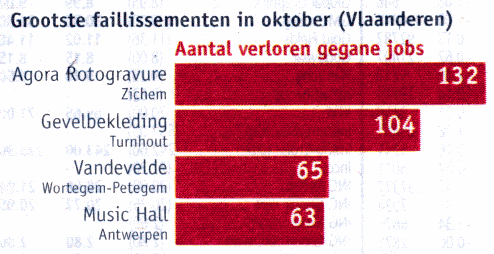
\includegraphics[width=0.6\textwidth]{horizontaal_staafdiagram-faillissementen}
\end{center}
\vraag{Welke veranderlijke is er genoteerd bij elke persoon die zijn job is
kwijtgeraakt? Welk soort veranderlijke is dat? Wat zijn haar waarden? Is de figuur goed
getekend?}
\pause
Voor elke persoon die zijn job is verloren, is genoteerd op welk bedrijf hij werkte. De
\uline{veranderlijke is hier “de bedrijfsidentificatie”}. Dat is een \uline{kwalitatieve
veranderlijke} met waarden: “Agora Rotogravure, Zichem”, “Gevelbekleding, Turnhout”,
“Vandevelde, Wortegem-Petegem”, en “Music Hall, Antwerpen”. De figuur is een
staafdiagram waarbij de \uline{volgorde van de staafjes bepaald is door de frequentie}. Dat is goed.
\end{frame}

\begin{frame}
\frametitle{Frequentietabel interpreteren}
\begin{columns}
\begin{column}{0.6\textwidth}
\vraag{Is “druggebruik” behandeld als een kwalitatieve veranderlijke? Is de tabel correct?}
\end{column}
\begin{column}{0.4\textwidth}
  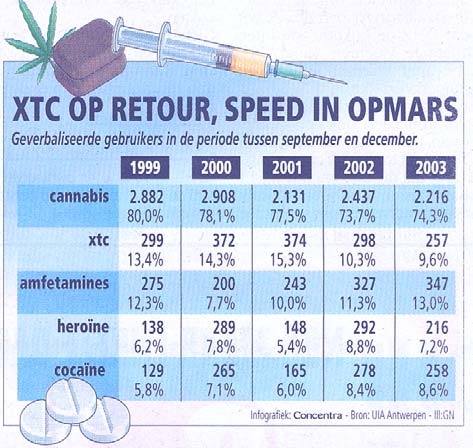
\includegraphics[width=\textwidth]{tabel-drugs}
\end{column}
\end{columns}
\pause
Drugs lijkt hier behandeld te zijn als een \uline{kwalitatieve veranderlijke} met
waarden: “cannabis”, “xtc”, “amfetamines”, “heroïne”, en “cocaïne”. De \uline{tabel is fout want het totaal van de percenten is 112.7\%}. Dit is zeker niet te
wijten aan afrondingsfouten, maar aan het feit dat sommige geverbaliseerden meerdere drugs namen en dus in meer dan één categorie zijn terechtgekomen.
\end{frame}

\begin{frame}
\frametitle{Taartdiagram interpreteren}
\begin{columns}
\begin{column}{0.6\textwidth}
\vraag{Is “vrijetijdsbesteding” hier behandeld als een kwalitatieve veranderlijke? Is het taartdiagram correct getekend?}
\end{column}
\begin{column}{0.4\textwidth}
  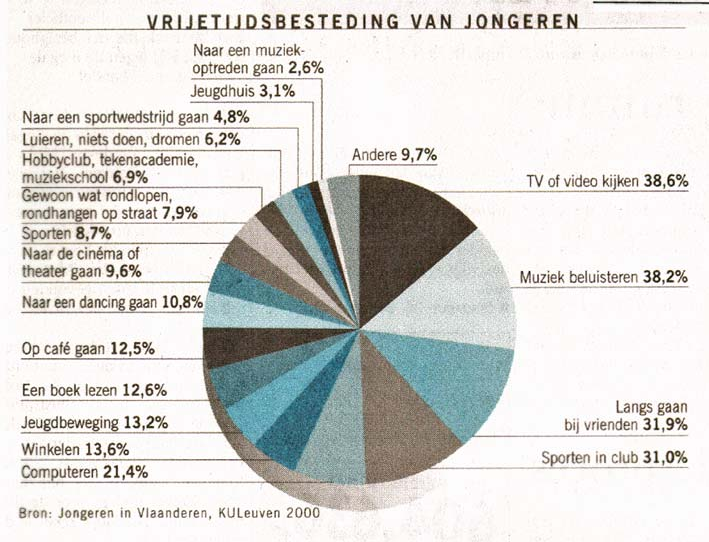
\includegraphics[width=\textwidth]{cirkeldiagram-vrijetijdsbesteding}
\end{column}
\end{columns}
\pause
Vrijetijdsbesteding lijkt in deze studie behandeld te zijn als een \uline{kwalitatieve veranderlijke} met waarden: “TV of video kijken”, “Muziek beluisteren”, “Langs gaan bij vrienden”, enz. Het taartdiagram volgt ook de klassieke afspraak om bovenaan te beginnen en dan naar rechts te draaien, met eerst de grootste sector, dan de tweede grootste, enz. Een uitzondering hierop is de laatste sector die 9.7\% bevat en “Andere” heet. Het is logisch dat je “Andere”(wat een allegaartje is van al wat overschiet) niet tussen de andere sectoren plaatst. Het \uline{taartdiagram is echter foutief want de volledige taart moet 100\% zijn en hier is dat 270\%}. Er is hier gewerkt met uitkomsten die elkaar overlappen.
\end{frame}

\begin{frame}
\frametitle{Statistisch onderzoek naar het schatten van de tijdsduur}
Hoe lang denken we dat één minuut duurt?
\begin{itemize}
  \item Wil je weten hoe één bepaalde leerling een minuut schat?
  \item Hoe schatten de leerlingen op je school dat één minuut duurt als ze maar éénmaal mogen schatten?
\end{itemize}
\pause
\vraag{Wat onderzoek je hier bij welke populatie?}
\pause
Ik onderzoek \uline{hoe lang leerlingen van mijn school de tijdsduur van één minuut schatten als zij
maar één keer de kans krijgen} om dit te doen.
\pause
\vraag{Eigenlijk geef je een kleine opdracht aan elke leerling uit je steekproef. Is het belangrijk dat
je vooraf vastlegt hoe die opdracht moet uitgevoerd worden? Wat is de afspraak die je maakt
om het onderzoek correct uit te voeren? Kan de plaats of het tijdstip van ondervragen
invloed hebben op de kwaliteit van de metingen?}
\pause
Elke leerling moet op \uline{dezelfde manier de opdracht uitvoeren}. Dat is belangrijk want anders
kunnen storende factoren (zoals lawaai in de klas) het \uline{resultaat beïnvloeden}. We hebben hier
afgesproken dat aan de leerling goed vooraf wordt uitgelegd hoe de test verloopt, dat hij
moet schatten met de ogen dicht en dat alle andere leerlingen stil moeten zijn.
\end{frame}

\begin{frame}
\frametitle{Dataset opstellen}
We stellen de dataset op. Veranderlijke is tijd. Hierop kunnen we wel wiskundige bewerkingen uitvoeren.\\
\vspace*{0.5cm}
\pause
{\bf kwantitatieve veranderlijke}: Veranderlijke weergegeven door een getal.\\
{\bf Continue kwantitatieve veranderlijke}: Veranderlijke kan alle mogelijke waarden aannemen tussen bepaalde grenzen.\\
{\bf Discrete kwantitatieve veranderlijke}: Tussen de mogelijke waarden zitten onderbrekingen.\\

\pause
\vraag{Schrijf alle gemeten waarden op.}
\end{frame}

\begin{frame}
\frametitle{Frequentietabel met klassenindeling}
{\bf frequentietabel met klassenindeling}.

\begin{center}
  \begin{tabular}{|c|c|}
    \hline
    Klasse & Frequentie\\
    \hline
    $[30;35[$ & $1$\\    
    \hline
    $[35;40[$ & $0$\\
    \hline
    $[40;45[$ & \ldots\\ 
    \hline
    \ldots & \ldots\\ 
    \hline
  \end{tabular}
\end{center}

Werkwijze:
{\scriptsize
\begin{itemize}
  \item Start met een interval dat groot genoeg is om al je opmetingen te kunnen bevatten.
  \item Op dit grote interval maak je nu deelintervallen die mooi aan elkaar aansluiten en elkaar niet
overlappen. Dat zijn je klassen.
  \item Elke klasse is een “links gesloten – rechts open” interval. De
grenzen van een klasse heten klassengrenzen. Het midden heet klassenmidden en de
breedte heet klassenbreedte.
  \item Zorg ervoor dat het overgrote deel van de waarnemingen niet binnen één of twee klassen
valt.
\end{itemize}
}

\pause
\begin{columns}
\begin{column}{0.6\textwidth}
{\bf Turven} is tellen door streepjes per vijf te groeperen.
\end{column}
\begin{column}{0.4\textwidth}
  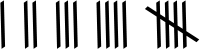
\includegraphics[width=0.6\textwidth]{turven}
\end{column}
\end{columns}
\end{frame}

\begin{frame}
\frametitle{Frequentietabel met klassenindeling (vervolg)}
\vraag{Stel nu een frequentietabel op voor jouw onderzoek. Je kan je laten leiden door bovenstaand
voorbeeld en de klassenbreedte gelijk aan 5 nemen, tenzij dat voor de data niet zinvol is.}
\begin{center}
  \begin{tabular}{|p{1.5cm}|p{1.5cm}|p{1.5cm}|p{1.5cm}|p{1.5cm}|p{1.5cm}|}
    \hline
    Klasse & Turf & Frequentie &&Rel. Freq&\\
    \hline&&&&&\\\hline&&&&&\\\hline&&&&&\\\hline&&&&&\\\hline&&&&&\\
    \hline&&&&&\\\hline&&&&&\\\hline&&&&&\\\hline&&&&&\\\hline&&&&&\\
    \hline&&&&&\\\hline&&&&&\\\hline&&&&&\\\hline
  \end{tabular}
\end{center}
\end{frame}

\begin{frame}
\frametitle{Cumulatieve frequenties}
{\it Cumulatief} wil zeggen dat iets steeds toeneemt of ophoopt.\\
\vspace*{0.5cm}
\pause
{\bf Cumulatieve frequentie}: het aantal gegevens dat tot deze klasse en alle lagere klassen behoord.\\
{\bf Relatieve cumulatieve frequentie}: van een klasse is de verhouding van de cumulatieve frequentie van die klasse en het totale aantal gegevens.

\vraag{Vul de frequentietabel verder aan met de cumulatieve frequentie en de relatieve cumulatieve frequentie.}
\end{frame}

\begin{frame}
\frametitle{Histogram}

{\bf Histogram:} meest gebruikte figuur om continu kwantitatieve gegevens weer te geven.

Werkwijze:
\begin{enumerate}
  \item Kies op de $x$-as een lengte-eenheid en breng op de $x$-as de beeldpunten van de klassengrenzen aan.
  \item De klassenfrequenties worden voorgesteld met behulp van rechthoeken die de horizontale lijnstukken op de $x$ as als zijde hebben. Dan moet de verticale zijde zo zijn, dat de oppervlakte van de bijbehorende rechthoek recht evenredig is met de frequentie van een klasse. We moeten dus de hoogte van elke rechthoek berekenen en vervolgens die rechthoeken construeren, allen aan de zelfde kant van de $x$-as.
\end{enumerate}

\vraag{Teken een histogram voor de opgestelde frequentietabel.}
\end{frame}

\begin{frame}
\frametitle{Kengetallen}
Informatie in enkele getallen samenvatten.\\
\vspace*{0.5cm}
\pause
De typische waarde, het getal dat het "centrum" van alle resultaten bevat:\\
\pause
gemiddelde, mediaan.\\
\vspace*{0.5cm}
\pause
Bij \underline{discrete kwantitatieve gegevens}:
\vraag{Bereken het gemiddelde van de volgende toetsresultaten: 4, 5.5, 6, 6, 6, 6.5, 7, 7, 7, 7.5, 7.5, 8, 8, 8, 8, 8.5, 8.5, 9, 9.5, 10, 10.}
\vspace*{1cm}
\pause
\vraag{Bereken de mediaan van de volgende toetsresultaten: 4, 5.5, 6, 6, 6, 6.5, 7, 7, 7, 7.5, 7.5, 8, 8, 8, 8, 8.5, 8.5, 9, 9.5, 10, 10.}
\vspace*{1cm}
\end{frame}
\begin{frame}


\frametitle{Kengetallen: gemiddelde}
Bij \underline{continue kwantitatieve gegevens}:\\
\begin{description}
\scriptsize
  \item[gemiddelde:] Zoek van elke klasse het klassenmidden, vermenigvuldigd dit met de bijhorende frequentie en noem dit het product, tel alle producten op, het gemiddelde is het quotient van die som en van de som van de frequenties.
\end{description}
\pause
\vraag{Bereken nu het gemiddelde.}
\begin{center}
  \begin{tabular}{|p{2cm}|p{3cm}|p{2cm}|p{2cm}|}
    \hline
    Klasse & Klassenmidden & Frequentie & Product\\
    \hline&&&\\\hline&&&\\\hline&&&\\\hline&&&\\\hline&&&\\
    \hline&&&\\\hline
    \multicolumn{2}{r|}{Som:} & &\\\cline{3-4}
  \end{tabular}
\end{center}
Het gemiddelde is:
$$
\bar{x}=\frac{\phantom{.......................}}{\phantom{.....................}}=
$$
\vspace*{0.5cm}
\end{frame}

\begin{frame}
\frametitle{Kengetallen: mediaan}
Bij \underline{continue kwantitatieve gegevens}:\\
\begin{description}
\scriptsize
  \item[mediaan:] Gegevens ordenen van klein naar groot en kijken in welke klasse de middelste waarde zich bevind.
\end{description}
\pause
\vraag{Bepaal de mediaan van ons onderzoek.}
\vspace*{10cm}
\end{frame}

\begin{frame}
\frametitle{Kengetallen: standaardafwijking en interkwartielafstand}
Spreiding rond het centrum:\\
\pause
\begin{description}
  \item[Standaardafwijking ($s$)] Spreiding rond het gemiddelde.\\
  Een te gekke formule! We zullen deze altijd met software berekenen.
  \pause
  \item[Interkwartielafstand (IQR)] Spreiding rond de mediaan.\\
  De lengte van het gebied waarin de middelste 50\% van de geordende opmetingen liggen. Als we de reeds berekende mediaan Q2 noemen, dan is Q1 te bepalen door de mediaan te nemen van de gegevens links van Q2 en Q3 is te bepalen door de mediaan te nemen van de gevens rechts van Q2. Ook dit kengetal zullen we berekenen met software.
\end{description}
\end{frame}

\begin{frame}
  \frametitle{Boxplot}
  De {\bf boxplot} geeft ons een goed zicht op zowel het centrum als de spreiding van je opmetingen.\\
  Werkwijze:
  \begin{itemize}
    \item Linkerstaart: vanaf de kleinste meting die groter of gelijk is aan $\mbox{Q1} - (1.5\cdot\mbox{IQR})$ tot Q1, elke kleinere observatie is een uitschieter en duiden we apart aan.
    \item Linkerrechthoek: van Q1 tot Med (de mediaan of Q2).
    \item Rechterrechthoek: van Med tot Q3.
    \item Rechterstaart: van Q3 tot aan de grootste opmeting die kleiner of gelijk is aan $\mbox{Q3} + (1.5\cdot\mbox{IQR})$. Elke observatie die nog groter is, wordt als een uitschieter beschouwd en apart aangeduid.
  \end{itemize}
\pause
\vraag{Teken nu de boxplot van het onderzoek. Vergeet de x-as niet te voorzien van de juiste getallen en de juiste
eenheid.}
\pause
\vraag{Zijn er uitschieters in je dataset? Was dat te verwachten?}
\pause
Misschien, dit is vooraf moeilijk in te schatten.
\end{frame}

\begin{frame}
\frametitle{Vertekende resultaten}
Als al je opmetingen op een systematische manier te klein (of te groot) zijn dan heb je {\bf vertekening}.\\
\vspace*{0.5cm}
\pause
\vraag{Als je een weegschaal moet gebruiken waarvan je vermoedt dat zij systematisch een te laag gewicht
aangeeft, hoe zou jij dan een boekentas daarop wegen, als je met die weegschaal vooraf niets
mag doen?}
\pause
{
Als je het \uline{verschil maakt van twee dingen die beide evenveel “vertekend” zijn, dan valt die
vertekening weg}. Zet dus niet die boekentas op de weegschaal, maar neem die in je hand en
ga er mee op de weegschaal staan. Bepaal daarna je gewicht zonder boekentas op diezelfde
weegschaal. Maak dan het verschil en je hebt het “goede” gewicht van die boekentas.}
\pause
\vraag{Je moet de lengte van 20 planken meten en je doet dat met een rolmeter. Op welke manier
zou hier vertekening kunnen optreden?}
\pause
Elke “systematische” fout die op die rolmeter kan zitten zorgt voor vertekening. Zo kan
\uline{bijvoorbeeld het metalen haakje aan het begin van de rolmeter scheef staan} zodat
systematisch één millimeter te weinig wordt afgelezen.
\end{frame}

\begin{frame}
\frametitle{Samenvatting van het onderzoek}
Je samenvatting bestaat uit twee delen
\begin{enumerate}
  \item De antwoorden op de contextvragen (de www-vragen),
  \item De besluiten over het uitgevoerde onderzoek.
\end{enumerate}
\pause
\vraag{Formuleer nu de antwoorden op de contextvragen (de www-vragen).}
\pause
Dit onderzoek is uitgevoerd in de maand \uline{april van 2012 in onze school}. \uline{Hoe de leerlingen van onze school de tijdsduur schatten} was onze onderzoeksvraag.  We hebben als \uline{steekproef de 17 leerlingen uit de klas} genomen. De leerlingen hebben wij de \uline{tijdsduur van één minuut laten schatten}. Voor het schatten van die minuut moest de geteste leerling de ogen sluiten, en het moest stil zijn in de klas. Wij hebben \uline{de tijdsduur genoteerd tot op de seconde}.
\pause
\vraag{Formuleer nu de besluiten over het uitgevoerde onderzoek.}
Gemiddelde, mediaan, besluit ivm. centrummaten. Uitzicht histogram. Spreiding rond gemiddelde? rond mediaan?. Zijn er uitschieters?
\end{frame}

\begin{frame}
\frametitle{Zelfevaluatie}
In dit onderzoek heb je geleerd over:
\begin{itemize}
  \item vertekening bij opmetingen
  \item de continu kwantitatieve veranderlijke
  \item de frequentietabel met klassenindeling
  \item het histogram en de boxplot
  \item het gemiddelde en de mediaan
  \item de standaardafwijking en de interkwartielafstand
  \item de interpretatie van kengetallen in combinatie met grafieken
\end{itemize}
\end{frame}

\begin{frame}
\frametitle{Vragen}
\vraag{Wanneer is een kwantitatieve veranderlijke continu? Zeg dat in je eigen woorden, en geef enkele voorbeelden.}
\pause
Een kwantitatieve veranderlijke is continu als er tussen gelijk welke twee mogelijke waarden nog andere mogelijke waarden kunnen zijn. Er zijn dus geen sprongen in de mogelijke uitkomsten van de veranderlijke (eventueel zie je wel sprongen in de opmetingen omdat de meetapparatuur niet fijn genoeg kan meten). Afstand, gewicht, tijd... zijn continu kwantitatieve veranderlijken. Het aantal auto’s in een gezin is discreet kwantitatieve veranderlijken.
\pause
\vraag{Schrijf je een continu kwantitatieve veranderlijke altijd op met kommagetallen? Motiveer je
antwoord.}
\pause
Of je de waarde van een continu numerieke veranderlijke opschrijft met decimalen, heeft te maken met de keuze van de eenheid en niet met de aard van de veranderlijke. Een afstand van $2.25$ meter kan je ook opschrijven in centimeter. Dat wordt dan $225$ cm, en nu zijn de decimalen plots weg!
\end{frame}

\begin{frame}
\frametitle{Vragen}
\vraag{Welke eigenschap probeert de standaardafwijking te beschrijven? Zeg in woorden hoe je de standaardafwijking berekent. Kan je daaruit afleiden of de standaardafwijking gevoelig is voor uitschieters? Kan je daarvan een eenvoudig voorbeeld geven?}
\pause
{\scriptsize
De \uline{standaardafwijking is een maat voor de afwijking van een verzameling getallen ten opzichte van hun gemiddelde}. Als getallen ver uitgespreid liggen rond hun gemiddelde dan is de standaardafwijking groot. Als zij allemaal dicht tegen het gemiddelde liggen dan is de standaardafwijking klein.\\
De formule voor de standaardafwijking, die ik overschrijf uit de werktekst, is:
$$
s = \sqrt{\frac{1}{n-1}\sum^n_{i=1}(x_i - \bar{x})^2}
$$
In deze uitdrukking zie ik dat je begint met te kijken hoeveel elke opmeting $x_i$ afwijkt van het
gemiddelde $\bar{x}$ . Het verschil tussen $x_i$ en $x$ wordt gekwadrateerd en dan maak je de som van
al die gekwadrateerde verschillen. Die som wordt gedeeld door $(n–1)$ en uit dat resultaat
trekt men de vierkantswortel.\\
Elke observatie $x_i$ speelt een rol in deze formule, en een uitzonderlijk grote $x_i$ (zoals een
uitschieter) geeft een heel grote
$$
(x_i - \bar{x})^2
$$
waarde, zodat ook $s$ groter wordt. De standaardafwijking is dus duidelijk \uline{gevoelig voor uitschieters}.
}
\end{frame}

\begin{frame}
\frametitle{Vragen}
\vraag{Welke eigenschap probeert de interkwartielafstand te beschrijven? Zeg in woorden wat kwartielen zijn en hoe je de interkwartielafstand berekent. Kan je daaruit afleiden of de interkwartielafstand gevoelig is voor uitschieters? Kan je daarvan een eenvoudig voorbeeld geven?}
\pause
{\scriptsize
De interkwartielafstand is een maat voor de spreiding van getallen. Hij geeft aan binnen welk gebied rond de mediaan de middelste helft van al je gegevens liggen. Als de IQR klein is, dan liggen die gegevens dicht rond de mediaan geconcentreerd, en als hij groot is dan liggen die data verder uiteen.\\
Kwartielen zijn waarden die de geordende getallenrij in kwartjes verdelen. Zij worden bepaald op een analoge manier zoals de mediaan, maar dan afzonderlijk voor de onderste helft en de bovenste helft van de dataset. De mediaan van de onderste helft is het eerste kwartiel Q1, en de mediaan van de bovenste helft is het derde kwartiel Q3 . De afstand tussen die twee kwartielen is de interkwartielafstand.\\
Als je de waarden van het kleinste kwart getallen nog verkleint (of van het grootste kwart nog vergroot) veranderen Q1 en Q3 niet, en dus is de interkwartielafstand niet gevoelig voor uitschieters.\\
Als er bij getallen die allemaal rond 20 liggen één tikfout optreedt, zoals 17, 18, 19, 20, 21,
22, 2333 in plaats van 17, 18, 19, 20, 21, 22, 23 dan verandert de IQR niet.
}
\end{frame}

\begin{frame}
\frametitle{Projecten}

\begin{center}
{\Huge Nu is het aan jou!}
\end{center}
%\\ Kies zelf een project en voer een statistisch onderzoek uit.

\end{frame}



\end{document}
%%%%%%%%%%%%%%%%%%%%%%%%%%%%%%%%%%%%%%%%%%%%%%%%%%%%%%%%%%%%%%%%%%%%%%%%%%%%%%%%%%%%%%%%%

\begin{frame}
\frametitle{}
\end{frame}


\begin{columns}
\begin{column}{0.6\textwidth}

\end{column}
\begin{column}{0.4\textwidth}
  \includegraphics[width=\textwidth]{}
\end{column}
\end{columns}






















